\newpage
\section{Per-sequence Sampling Reduces Loss Spikes}
\label{sec:loss-spikes}

When running our per-sequence sampling experiments, we observed that the training curves of per-sequence sampling helped eliminate loss spikes during training. Specifically, in \cref{fig:per-sample-training}, for our 350M parameter Parcae models, per-micro-batch has several loss spikes through training while per-sequence sampling does not. We can observe from \cref{fig:residual-state-norm}, that these training spikes stem directly from overly large recurrent residual jumps at the final recurrence, implying the model is not learning to converge to a steady-state fixed point solution. 
It can then be observed that per-sequence depth helps provide a better estimate for our training objective, enabling convergent fixed-point behavior and preventing loss-spikes during training. The direct benefit of this can be observed in \cref{tab:training-res}, where per-sequence sampling significantly improves the downstream quality of looped models, especially at low test-time recurrences. Finally, we note that per-sequence sampling adds a minimal amount of training overhead, increasing total wall clock time for pretraining by 1.8\%, which we believe can be further optimized away with a cleaner implementation.

\begin{figure}[!ht]
    \centering
    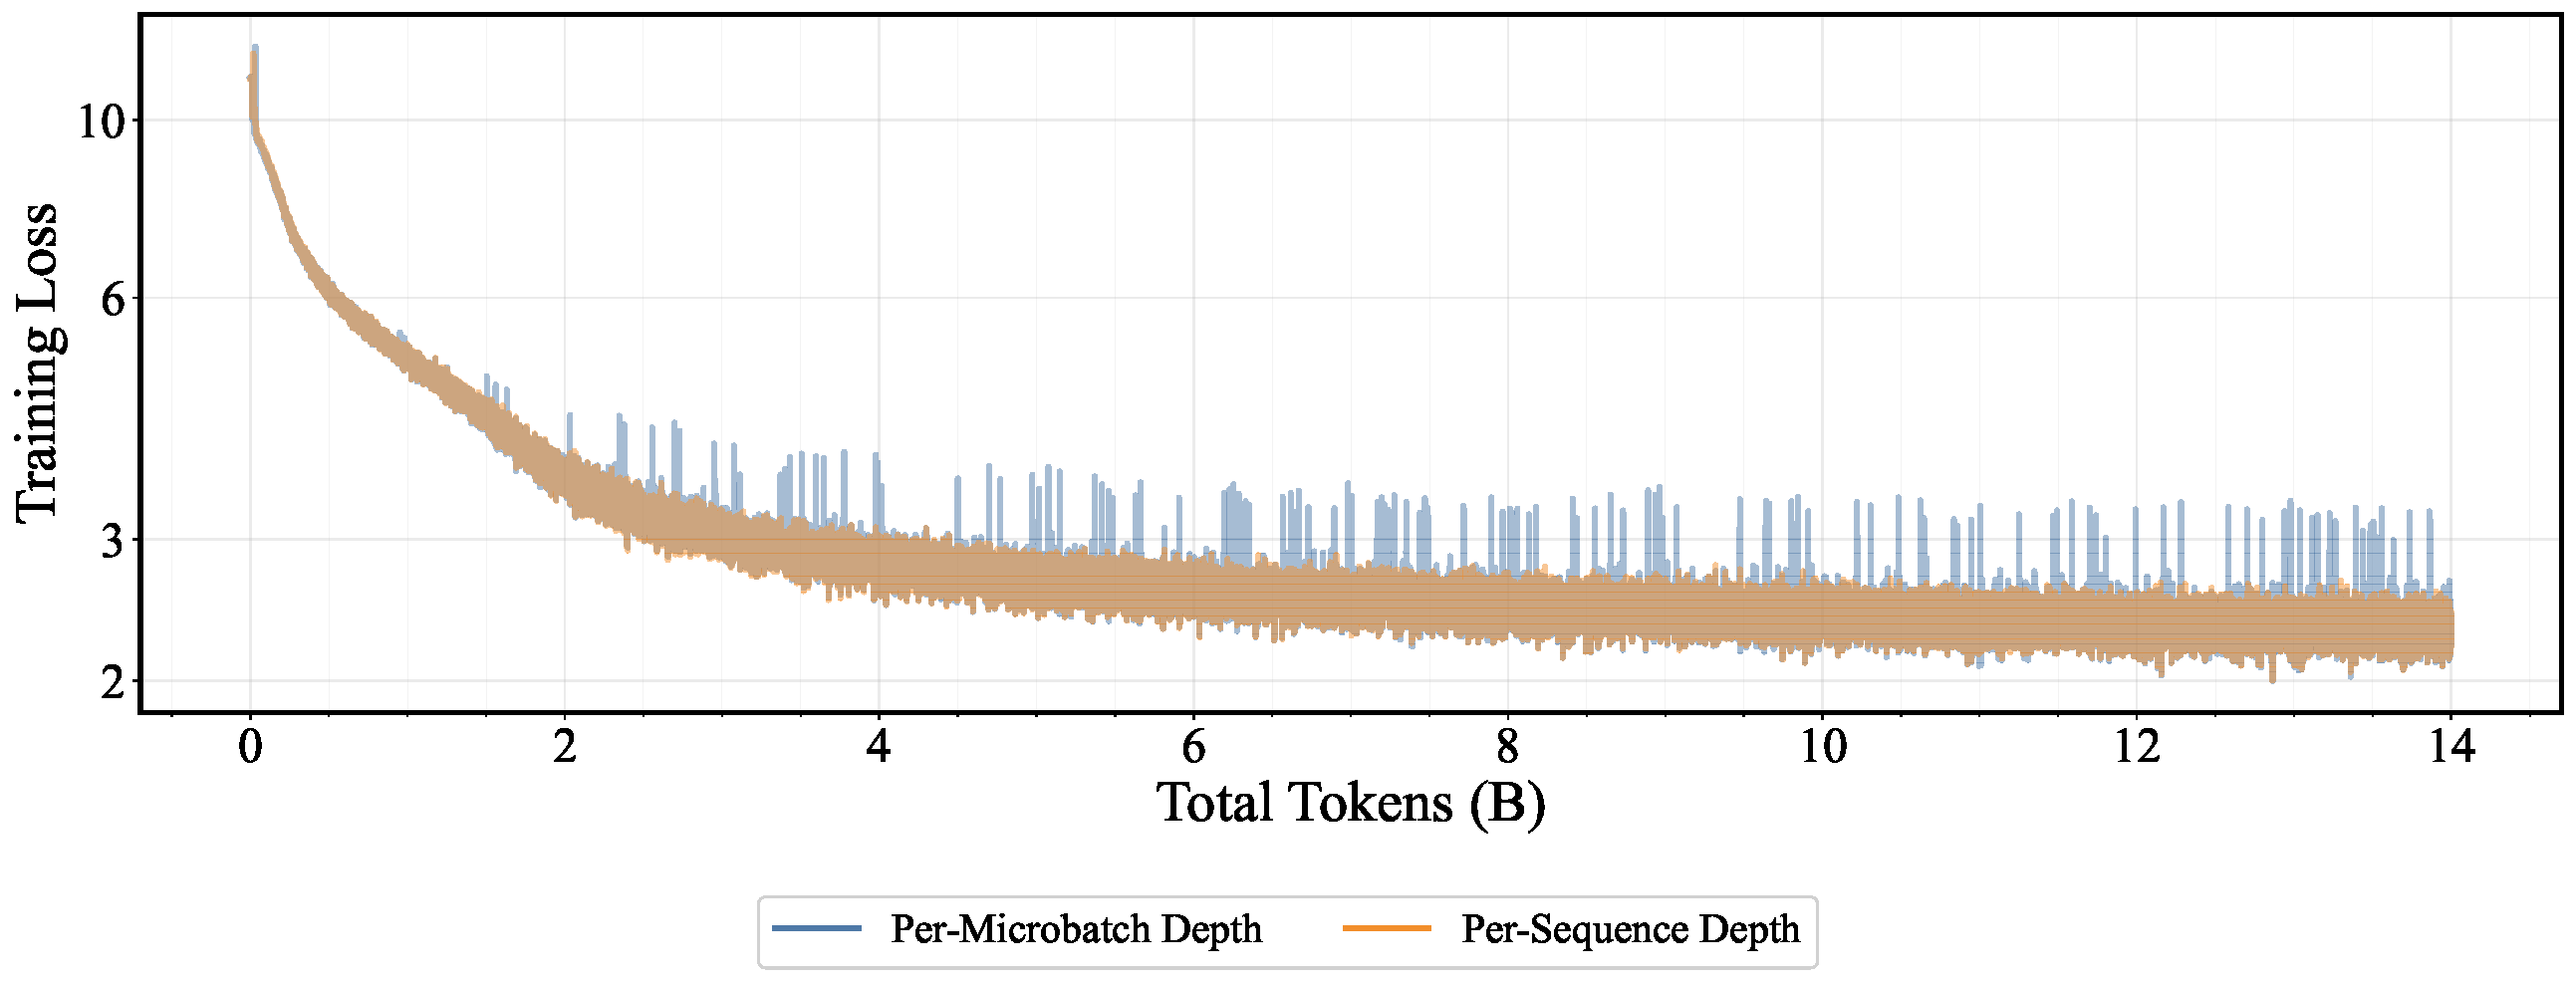
\includegraphics[width=\linewidth]{figures/appendix/stochastic_depth_350m_training_loss.pdf}
    \vspace{-2.5em}
    \caption{Training curves showing per-sequence sampling effectively eliminates loss spikes in training over per-micro-batch sampling.}
    \label{fig:per-sample-training}
\end{figure}

\begin{figure}[!ht]
    \centering
    \vspace{-1.5em}
    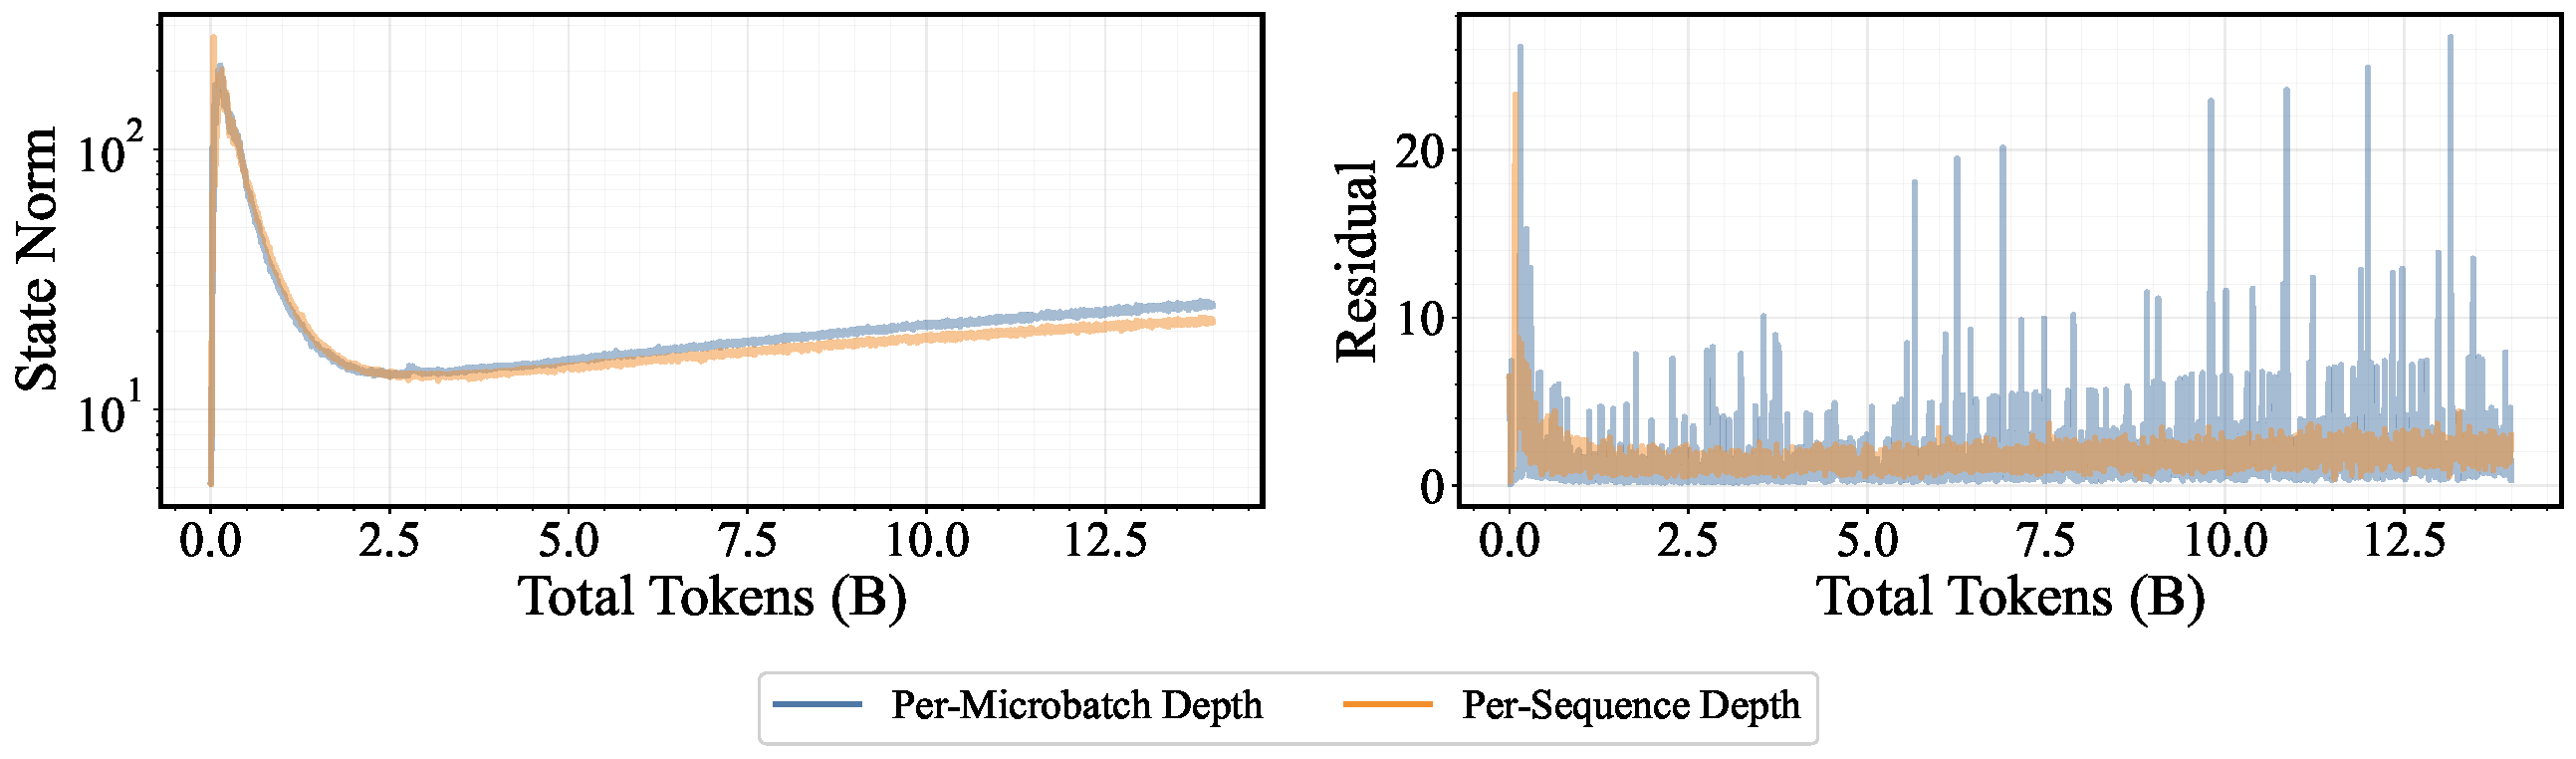
\includegraphics[width=\linewidth]{figures/appendix/stochastic_depth_350m_norm_residual.pdf}
    \vspace{-2em}
    \caption{Comparison of recurrent residual and state norm metrics (defined in \cref{sec:notation}), which show that per-sequence sampling enables stronger fixed point behavior in training.}
    \label{fig:residual-state-norm}
\end{figure}

\begin{table}[!ht]
        \vspace{0pt}
        \small
        \renewcommand{\arraystretch}{1.2} 
        \centering
        \begin{tabular}{@{}lccccc@{}}
        \toprule
        & \textbf{Method} & \textbf{T=1} & \textbf{T=4} & \textbf{T=8} & \textbf{T=16} \\
        \midrule
        \multirow{2}{*}[0pt]{\rotatebox{90}{\small{100M}}} & Per-Batch & 300.32 & 36.75 & 16.65 &  13.81 \\
                                                    & Per-Sequence & \textbf{70.47} & \textbf{17.15} & \textbf{14.08} &  \textbf{13.59} \\
        \midrule
        \multirow{2}{*}[0pt]{\rotatebox{90}{\small{350M}}} & Per-Batch & 167.61 &  12.80 &  10.40 &  10.24  \\
                                                    & Per-Sequence & \textbf{17.92} & \textbf{10.49} &  \textbf{10.09} &  \textbf{10.11} \\
        \bottomrule
        \end{tabular}
        \caption{\textbf{Per-Microbatch vs. Per-Sequence Comparison}. We compare perplexity of Parcae models trained with per-microbatch sampling \citep{geiping_scaling_2025} and per-sequence sampling, using different recurrences ($T$) on a held-out validation set. \textbf{Bolded} results indicate \textbf{best} at each scale.}
        \label{tab:training-res}
\end{table}
